\documentclass{article}
\usepackage{quad}

\hypersetup{pdftitle={Trees meet octahedron comparison},
pdfauthor={Nina Lebedeva and Anton Petrunin}}

\newcommand{\Addresses}{{\bigskip\footnotesize

\noindent Nina Lebedeva,
\par\nopagebreak
 \textsc{Saint Petersburg State University, 7/9 Universitetskaya nab., St. Petersburg, 199034, Russia}
\par
\nopagebreak
 \textsc{St. Petersburg Department of V.A. Steklov Institute of Mathematics of the Russian Academy of Sciences, 27 Fontanka nab., St. Petersburg, 191023, Russia}
  \par\nopagebreak
  \textit{Email}: \texttt{lebed@pdmi.ras.ru}

\medskip

\noindent   Anton Petrunin, 
\par\nopagebreak
 \textsc{Math. Dept. PSU, University Park, PA 16802, USA.}
  \par\nopagebreak
  \textit{Email}: \texttt{petrunin@math.psu.edu}
  
}}

\begin{document}
%\pagestyle{empty}\renewcommand\includegraphics[2][{}]{}


\title{Trees meet octahedron comparison}
\author{Nina Lebedeva and Anton Petrunin}

\date{}
\maketitle
\begin{abstract}
We show that trees and their products meet octahedron comparison.
\end{abstract}

Let us recall the definition of \emph{graph comparison} given by Vladimir Zolotov and the authors \cite{lebedeva-petrunin-zolotov}.

Let $\Gamma$ be a graph with vertices $v_1,\dots,v_n$.
A metric space $X$ is said to meet the $\Gamma$-comparison if for any set of points in $X$ labeled by vertices of $\Gamma$ there is a model configuration $\tilde v_1,\dots,\tilde v_n$ in the Hilbert space $\HH$ such that 
if $v_j$ is adjacent to $v_j$, then
\[|\tilde v_i-\tilde v_j|_{\HH}\le | v_i-v_j|_{X}\]
and
if $v_j$ is nonadjacent to $v_j$, then
\[|\tilde v_i-\tilde v_j|_{\HH}\ge | v_i-v_j|_{X};\]
here $|p-q|_M$ denotes the distance between points $p$ and $q$ in the metric space~$M$.

\begin{wrapfigure}[9]{r}{35 mm}
\vskip-2mm
\centering
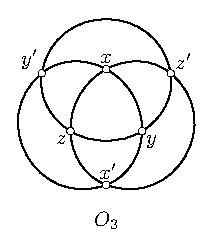
\includegraphics{mppics/pic-30}
\end{wrapfigure}

Let us denote by $O_3$ is the graph of octahedron shown on the diagram.

\begin{thm}{Theorem}
The $O_3$-comparison holds for products of metric trees.
\end{thm}

Note that the 4-cycle $C_4$ is an induced subgraph of $O_3$.
It follows that $O_3$-comparison implies $C_4$-comparison;
the latter is equivalent to $\CAT(0)$-comparison.
The converse does not hold in general, but the following question remains open.

\begin{thm}{Question}
Is it true that $O_3$-comparison holds in any complete length $\CAT(0)$ space?
\end{thm}

\parit{Proof of the theorem.}
First, let us show that $O_3$-comparison holds for any metric tree.
Consider a six-point configuration $x,y,z,x',y',z'$ in a tree labeled by the vertices of $O_3$ on the diagram.
We can assume that the union of geodesics $[xx']$, $[yy']$, and $[zz']$ is connected.
Indeed, suppose $[xx']$ does not intersect $[yy']$, and $[zz']$.
Then we can shrink to a point a geodesic $\gamma$ that minimizes the distance from $[xx']$ to $[yy']\cup[zz']$;
in the obtained tree $T'$ the distances $|x-x'|$, $|y-y'|$ and $|z-z'|$ remain the same and the remaining distances between $x,y,z,x',y',z'$ cannot get longer, so any model configuration for the six points in $T'$ works for the corresponding points in $T$.

Consider the union of intersections 
\[Y=([xx']\cap [yy'])\cup([yy']\cap [zz'])\cup([zz']\cap [xx']).\]
The remaining proof of this part splits into two cases:
\begin{enumerate}
\item The set $Y$ is a \emph{tripod}; that is, $Y$ is a union of three geodesics meeting at one point. 
\item $Y$ lies in one of the  geodesics $[xx']$, $[yy']$, or $[zz']$; in this case we may assume that $Y\subset [xx']$ without loss of generality.
\end{enumerate}

\parit{Case 1.}
Suppose $Y$ is a tripod; denote its center by $o$.
Without loss of generality, we may assume that geodesics $[xx']$, $[yy']$ and $[zz']$ have opposite orientattion on the overlaps.
Note that we can assume that in each pair $([ox],[oy'])$, $([oy],[oz'])$, and $([oz],[ox'])$ one of the geodesics lies in the other.
Indeed, assume it is not true, say $[ox]\not\subset[oy']$ and $|o-x|_T\le |o-y'|_T$.
Then moving $x$ to a point on $[oy']$ on the distance $|o-x|_T$ from $o$ will decrease the distance $|x-y'|_T$ and the rest of 14 distances between $x,y,z,x',y',z'$ will remain the same.
Therefore if a model configuration exists for the new configuration, then the same holds for the old one. 

If $[ox]\subset [oy']$, then set $a=x$, otherwise $a=y'$.
Similarly, chose  $b$ from $y$ or $z'$ and $c$ from $z$ or $x'$.
Consider model triangle $[\tilde a\tilde b\tilde c]$ of $[abc]$.

Note that $[ab]\subset [yy']$, $[bc]\subset [zz']$, and $[ac]\subset [xx']$.
Therefore we may choose points $\tilde x$, $\tilde x'$ on the lie $\tilde a\tilde c$ so that the map $x\mapsto \tilde x$, $x'\mapsto \tilde x'$, $a\mapsto \tilde a$, $c\mapsto \tilde c$ is distance-preserving.
Similarly we may choose $\tilde y$, $\tilde y'$ on the line $\tilde a\tilde b$ and $\tilde z$, $\tilde z'$ on the lie $\tilde b\tilde c$.
\begin{figure}[ht!]
\centering
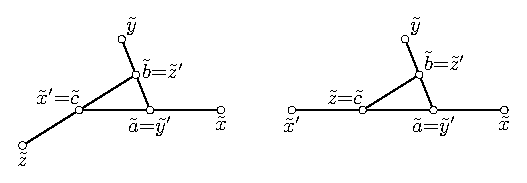
\includegraphics{mppics/pic-50}
\end{figure}
Couple of possible configurations are shown on the diagram.
The triangle inequality implies that the obtained configuration meets the required conditions.

\parit{Case 2.}
Suppose $Y\subset [xx']$.
Then $[yy']$ and $[zz']$ intersect $[xx']$ along two subsegments.
Without loss of generality, we may assume that $|x-y'|_T\ge |x-y|_T$ and $|x-z'|_T\ge |x-z|_T$;
in other words, geodesics $[xx']$, $[yy']$, and $[zz']$ oriented the same way on their overlaps.

In this case, the configuration $\tilde x,\tilde x',\tilde y,\tilde y',\tilde z,\tilde z'$ on a line described by their coordinates
\begin{align*}
\tilde x&=0,
&
\tilde y&=|y'-x|-|y'-y|,
&
\tilde z&=|z'-x|-|z'-z|,
\\
\tilde x'&=|x'-x|,
&
\tilde y'&=|y'-x|,
&
\tilde z'&=|z'-x|.
\end{align*}
It is straightforward to check that this configuration meets the conditions. 

\parit{Final step.}
It remains to show that $O_3$-comparison holds for a product of trees $\Pi\z=T_1\times \dots\times T_n$.
Any six-point configuration $x,y,z,x',y',z'\in \Pi$ can be described by $n$ six-point configurations $x_i$, $y_i$, $z_i$, $x'_i$, $y'_i$, $z'_i\in T_i$ for each $i$.
Choose a model configuration $\tilde x_i,\tilde y_i,\tilde z_i,\tilde x'_i,\tilde y'_i,\tilde z'_i\in \HH$ for each $i$.
Observe that the $n$-tuples $\tilde x=(\tilde x_1,\dots, \tilde x_n),\z\dots,\tilde z'=(\tilde z_1,\dots, \tilde z_n)$ in $\HH=\HH^{\times n}$ form a model configuration of $x,y,z,x',y',z'$.
\qeds



{\sloppy
\printbibliography[heading=bibintoc]
\fussy
}

\Addresses
\end{document}
